% Chapter 1

\chapter{Introducción general} % Main chapter title

En este capítulo se presentan conceptos básicos sobre la temática. También se comenta el contexto y las motivaciones que impulsan la realización de este proyecto. Además se menciona el alcance y los objetivos, y se analiza el estado del arte en el campo de estudio.

\label{Chapter1} % For referencing the chapter elsewhere, use \ref{Chapter1} 
\label{IntroGeneral}

%----------------------------------------------------------------------------------------

% Define some commands to keep the formatting separated from the content 
\newcommand{\keyword}[1]{\textbf{#1}}
\newcommand{\tabhead}[1]{\textbf{#1}}
\newcommand{\code}[1]{\texttt{#1}}
\newcommand{\file}[1]{\texttt{\bfseries#1}}
\newcommand{\option}[1]{\texttt{\itshape#1}}
\newcommand{\grados}{$^{\circ}$}

%----------------------------------------------------------------------------------------

%\section{Introducción}

%----------------------------------------------------------------------------------------
\section{Introducción}

El objetivo de este proyecto es desarrollar un modelo de inteligencia artificial prototipo que estime la temperatura del agua que circula en un equipo utilizado para la inducción de hipotermia a pacientes neonatales. Además se hará foco en la incidencia de los parámetros que se disponen en el cálculo para aportar al conocimiento sobre estos tratamientos. Esto puede significar a futuro una mejora en un producto que desarrolla la empresa y brindar a quienes necesiten este tratamiento un desarrollo superador del mismo respecto a la actualidad. El proyecto será desarrollado dentro del marco del programa de vinculación. 

La empresa es AmrrA y los equipos en cuestión tienen el nombre Amrraterm HTF. Estos sistemas se utilizan con el propósito de inducir una hipotermia controlada en pacientes neonatales. Existen contextos en los cuales esto proporciona una mejor evolución de los pacientes. El principal caso de uso es el de pacientes que sufren hipoxia al nacer, esto es, falta de oxígeno en el cerebro. En estos casos, a temperatura corporal normal la interacción entre las neuronas es alta y se pueden desarrollar efectos adversos en la capacidad cerebral del paciente. Por esto un tratamiento estándar es el de inducir hipotermia por 72 horas a fin de minimizar los efectos que la hipoxia puede generar a futuro en los pacientes. 

Para lograr esto el procedimiento estándar es sedar al paciente y colocarlo dentro de una incubadora, donde es envuelto en las mantas que forman parte del equipo. Por estas mantas circula agua destilada. El equipo recibe como dato de entrada la temperatura objetivo a la cual se quiere llevar al paciente, que suele ser de 33,5º C, y regula la temperatura del agua en función de la temperatura objetivo y la actual del paciente. Una vez terminado el tratamiento de hipotermia, el equipo funciona en un modo llamado rampa, en el cual sube paulatinamente la temperatura hasta llegar a un estado normal.

En la actualidad la temperatura del agua es regulada por un algoritmo de lógica difusa. En un rango de pesos estándar de los pacientes (entre 2,5 kg y 3,5 kg) el algoritmo funciona correctamente, pero es posible que en pesos inferiores o superiores haya comportamientos que este proyecto pueda mejorar. Se desarrollará este modelo para evaluar si funciona mejor que el algoritmo actual en ese rango, en los valores inferiores o en los superiores de peso. 

Se utilizarán diversos datos para construir un modelo acorde al problema como el peso del paciente, la edad, la temperatura objetivo y las variaciones de temperatura del agua y paciente. Además de construir un modelo superador, también se busca detectar la incidencia de ciertos parámetros, como el peso del paciente, que no se utiliza por el algoritmo actual. Para evaluar el comportamiento del modelo se implementa un entorno que permita ingresar datos y visualizar la respuesta del modelo para los datos ingresados. 

El equipo consta de una interfaz mediante la cual el personal de salud indica los datos necesarios, un sistema de mantas y cañerías por las que circula agua destilada,  un sistema térmico con la responsabilidad de administrar la energía para que el agua esté a la temperatura indicada y un algoritmo de lógica difusa responsable de calcular la temperatura óptima del agua para el tratamiento. Un diagrama de esto se puede apreciar en la figura \ref{fig:actual-diagram}. 

\vspace{1cm}

\begin{figure}[htbp]
	\centering
	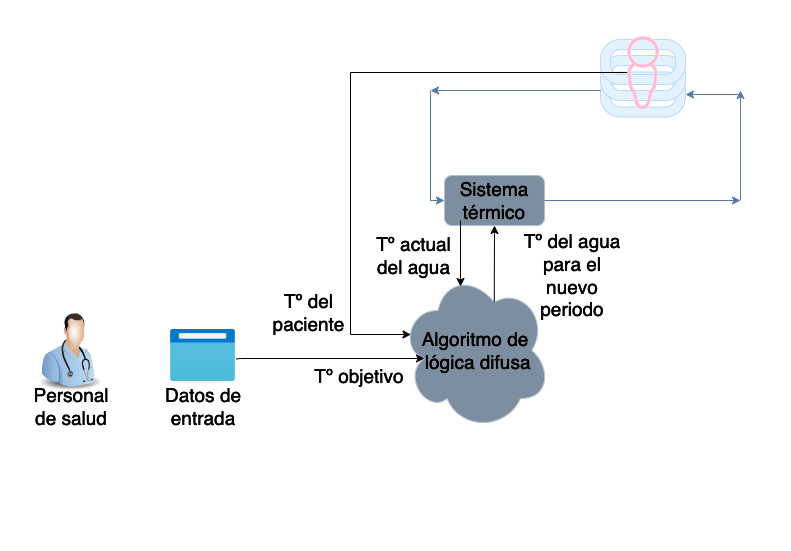
\includegraphics[width=1\textwidth]{./Figures/actual.png}
	\caption{Diagrama de funcionamiento del equipo.}
	\label{fig:actual-diagram}
\end{figure}

\vspace{1cm}

El modelo implementado cumple el mismo rol que el algoritmo que funciona actualmente, por lo que en el diagrama se lo puede ubicar a la par. Además de la temperatura objetivo, la actual del agua y la actual del paciente, recibirá el peso del paciente, y se compara el comportamiento de ambas soluciones. Se propone que funcionen un tiempo en paralelo y un elector defina cual de las temperaturas elegidas aplicar. Un diagrama de esto se puede apreciar en la figura \ref{fig:model-diagram}. 

\vspace{1cm}

\begin{figure}[htbp]
	\centering
	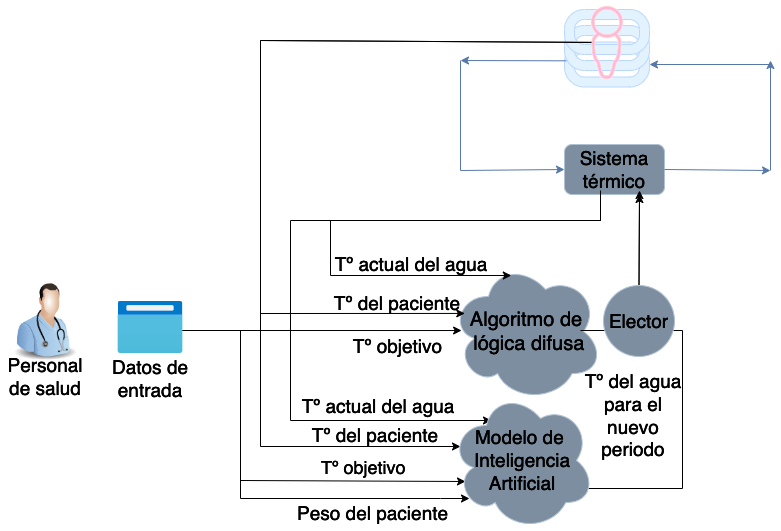
\includegraphics[width=1\textwidth]{./Figures/modelo.png}
	\caption{Diagrama del equipo con el nuevo modelo.}
	\label{fig:model-diagram}
\end{figure}

\vspace{1cm}

\section{Motivación}

Existen dos motivaciones fundamentales para el desarrollo de este proyecto. Por un lado, esta la incorporación de técnicas de inteligencia artificial para el modelado de tratamientos de inducción de hipotermia en los equipos mencionados, lo que supone una actualización al modelado actual y se puede esperar un comportamiento superador, lo que implicaría una mejor evolución en los pacientes. Por el otro, esta la incorporación del peso como variable para modelar el problema, lo que supone un mejor comportamiento y nuevamente, una mejoría en la evolución de los pacientes.
Sin embargo, es posible que el modelo resultante no se comporte mejor que el algoritmo actual. Estos equipos están en funcionamiento en una gran cantidad de hospitales en todo el país, y su funcionamiento es aceptado por la comunidad médica. En este caso, igual este proyecto aportará valor a la empresa, ya que brindará información acerca de la incidencia de los parámetros, y esto brindará un crecimiento en el conocimiento que se tiene sobre estos tratamientos.


\section{Conceptos generales}
A continuación mencionaremos la definición de algunos conceptos y valores importantes para la temática.
Como se mencionó anteriormente, los equipos en cuestión se denominan Amrraterm HTF. Algunos son propiedad de la empresa y se alquilan en centros de salud, mientras que otros fueron adquiridos. Están en funcionamiento en hospitales públicos y privados. Su dominio es acotado al tratamiento de regulación de temperatura en pacientes neonatales, esto es, en recién nacidos. El principal caso de uso es el de provocar una hipotermia controlada en pacientes que sufren hipoxia al nacer. Para esto, el profesional establece una temperatura a la que quiere llevar al paciente. Esta temperatura la denominamos temperatura objetivo. 
Los tratamientos suelen durar 72 hs. aproximadamente. Existen tres etapas en este tiempo. La primera, llamada rampa hacia abajo, se da en los primeros minutos del tratamiento, periodo en el que se busca llevar la temperatura del paciente hacia la objetivo, producto de la circulación de agua fría por las mantas. En la segunda etapa prima la estabilidad, aquí el objetivo es mantener al paciente en la temperatura objetivo. En la última etapa, denominada rampa hacia arriba, producto de la circulación de agua con mayor temperatura en las mantas del equipo, el paciente recupera su temperatura normal.
Al establecer los parámetros del tratamiento, el profesional indica el peso del paciente. Este dato no es tenido en cuenta por el algoritmo actual pero si se utiliza para el entrenamiento de los modelos de este proyecto.
Los pacientes suelen estar en un peso superior a 2,5 kg e inferior a 3,5 kg. En porcentaje, el desvío de este valor no es despreciable.

Podemos distinguir los siguientes atributos:
\begin{itemize}
	\item Temperatura objetivo, a la que se quiere llevar al paciente.
	\item Temperatura del agua que circula por las mantas.
	\item Temperatura actual del paciente en un instante del tiempo.
	\item Peso del paciente.
\end{itemize}

Uno de los criterios de bondad de estos equipos es que, en la etapa estable, la temperatura del paciente diste lo mínimo de la temperatura objetivo. En la práctica se ve que la temperatura oscila sobre la temperatura objetivo, por lo que podemos decir que un modelo será mejor que el actual, en la etapa estable, si la amplitud de la oscilación sobre la temperatura objetivo es menor.

\section{Objetivos y alcance}
Para el presente proyecto se plantean objetivos funcionales y conceptuales. Desde el punto de vista funcional se busca el desarrollo de una solución de inteligencia artificial acorde al problema planteado, lo que significa un nuevo enfoque respecto a lo que utilizan actualmente, una actualización y una potencial mejora de su producto. Desde el lado conceptual, se busca entender la incidencia de los parámetros, con mayor énfasis en el peso y en el comportamiento del modelo respecto a pacientes de distinto peso.

Se definieron los siguientes requerimientos:

\begin{enumerate}
	\item Requerimientos funcionales:
	\begin{enumerate}
		\item El modelo debe predecir el cambio de temperatura óptimo a aplicar.
		\item La salida del modelo debe ser conceptualmente análoga a la del algoritmo de lógica difusa utilizado actualmente, a fin de poder compararlos.
		\item El modelo debe dar una respuesta en un tiempo promedio menor o igual a 10 veces el tiempo promedio de respuesta del algoritmo actual.
		\item El sistema debe permitir ingresar datos de forma manual y mostrar el resultado.
		\item Se debe calcular la incidencia del peso y de los demás atributos en la solución.
	\end{enumerate}
	\item Requerimientos conceptuales:
	\begin{enumerate}
		\item Deben utilizarse datos sintéticos en las pruebas.
	\end{enumerate}
	\item Requerimiento de testing:
	\begin{enumerate}
		\item Se deben ejecutar pruebas secuenciales con datos reales y mostrar una comparación entre los resultados del modelo a implementar y del algoritmo actual.
		\item Se deben comparar tiempos entre el modelo propuesto y el algoritmo actual.
		\item Se debe calcular una métrica a definir para calcular la performance del modelo.
	\end{enumerate}
	\item Requerimiento de documentación:
	\begin{enumerate}
		\item Se deben documentar las decisiones tomadas.
		\item Se deben documentar los resultados de las pruebas y las distintas métricas.
		\item Se requiere documentar el código y las formas de utilizar al sistema.
	\end{enumerate}
	\item Requerimiento asociados con regulaciones
	\begin{enumerate}
		\item Se requiere que los casos utilizados no expongan datos que infrinjan derechos de privacidad.
	\end{enumerate}
\end{enumerate}


El proyecto no incluye: 
\begin{itemize}
	\item La incorporación del modelo a los equipos en funcionamiento.
	\item El despliegue del modelo en la nube.
	\item El desarrollo de una interfaz gráfica, una aplicación o una web.
\end{itemize}

\section{Estado del arte}

En el artículo \citep{jcm12062095} se habla acerca del tratamiento de inducción de hipotermia. Se mencionan estudios donde se realiza el tratamiento, valores seguros para el mismo y evolución de los pacientes. Esto puede ser útil para definir rangos de temperaturas adecuadas para el modelado del problema y tener mas conocimiento del contexto. Pero no se plantean soluciones de software para llevar a cabo los tratamientos.
Por otro lado están los artículos \citep{jcm12134434},	\citep{10.3389/fphys.2022.921884}, \citep{10125880}, \citep{doi:10.1177/09544119241266375} que analizan el uso de diversos modelos de \textit{machine learning} en contextos de hipotermia con el objetivo de predecir potenciales casos de hipotermia. También se analizó el articulo \citep{SHAMMI2022107013} que mediante inteligencia artificial busca predecir el daño causado por la hipotermia. Estos enfoques son interesantes para evaluar los riesgos de someter al paciente bajo este tratamiento pero no son el objetivo de este proyecto. En este caso el foco estará en un modelo que regule de forma óptima la inducción a hipotermia de un paciente. Por esto, sólo el primer artículo puede aportar información relevante al problema.

\begin{table}[h]
	\centering
	\caption[Estado del arte]{Comparación de lecturas encontradas}
	\begin{tabular}{l c c}    
		\toprule
		\textbf{Artículo} 	 & \textbf{Pacientes} 		& \textbf{Objetivo}  \\
		\midrule
 			\citep{jcm12062095} & Pediátricos 				&  Análisis de tratamientos de hipotermia\\		
			\citep{jcm12134434}   & General				& Predicción \\
 			\citep{10.3389/fphys.2022.921884} & Pediátricos 				&  Predicción\\		
			\citep{10125880} & General				& Predicción \\
			\citep{doi:10.1177/09544119241266375} 	 & General				& Predicción \\
			\citep{SHAMMI2022107013} & General				& Análisis de daño \\
		\bottomrule
		\hline
	\end{tabular}
	\label{tab:estado_del_arte}
\end{table}

